%
% teil1.tex -- Beispiel-File für das Paper
%
% (c) 2020 Prof Dr Andreas Müller, Hochschule Rapperswil
%
% !TEX root = ../../buch.tex
% !TEX encoding = UTF-8
%
\section{Herleitung
\label{schwimmen:section:naiver_weg}}
\kopfrechts{Problemstellung}

Hier ist eine Schritt für Schritt Darstellung der Herleitung zur optimalen Flussüberquerung dargestellt. Als Inspiration der Bilder und der Herangehensweise wurde an die Forumsfrage in \cite{schwimmen:mathForum} angelehnt. 

% papers/schwimmen/
\begin{figure}
    \centering
        \centering
        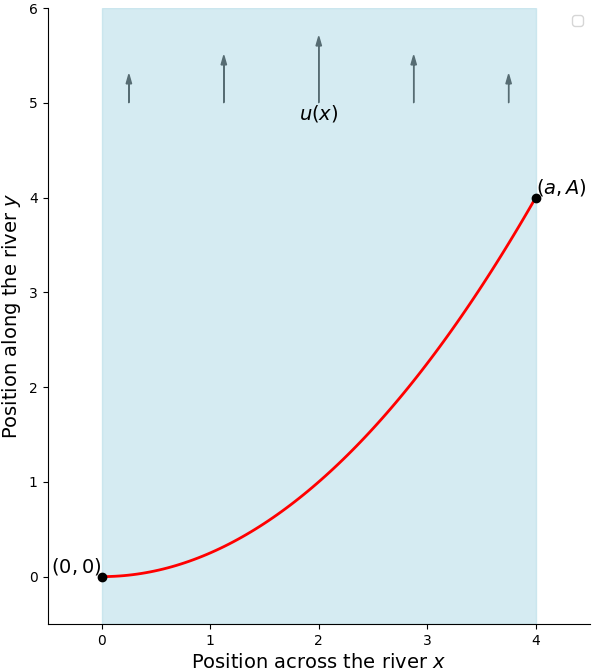
\includegraphics[width=0.6\textwidth]{papers/schwimmen/Grafiken/Figure_1-crop.png}	
        \caption{Fluss mit quadratischer Strömung. Ziel ist es von Punkt \((0,0)\) zum Punkt \((a,A)\) zu kommen, der am anderen Ufer liegt.}
        \label{fig:river_template}
\end{figure}

Ziel ist es die schnellste Route über den Fluss zu finden. In Abbildung \ref{fig:river_template} ist eine Flussüberquerung abgebildet, wobei \(a\) die Flussbreite ist und \(A\) die Distanz entlang des Flusses. Im Falle unserer Aufgabenstellung ist \(A=0\), da man am andern Ufer auf gleicher Höhe ankommt.

\subsubsection{Wichtige Kenngrössen}
Ein paar wichtige Kenngrössen für die Herleitung sind in Tabelle \ref{table:Wichtige_Kenngroessen} zufinden.

\begin{table}
    \centering
    \renewcommand{\arraystretch}{1.3}
    \begin{tabularx}{\textwidth}{@{}ll>{\raggedright\arraybackslash}p{7cm}@{}}
        \multicolumn{3}{c}{Wichtige Grössen} \\
        % \specialrule{.1em}{.05em}{.05em}
        % \textbf{Dataset} & \textbf{\(\mu\) in \(\mathrm{ps}\)} & \textbf{\(\sigma\) in \(\mathrm{ps}\)} \\
        \hline
        \(a\)   &   Flussbreite  &   definiert von der Umgebung \\
        \(c\)   &   Schwimmgeschwindigkeit        &   Definiert von der schwimmenden Person       \\
        \(u(x)\)   &   Flussgeschwindigkeit         &   Ist von der \(x\)-Position im Fluss abhängig     \\
        \((0,0)\)   &   Startpunkt         &   Startpunkt am Flussufer     \\
        \((a,A)\)   &   Endpunkt         &   Endpunkt auf anderer Ufer aber auf gleicher Höhe     \\
        \specialrule{.1em}{.05em}{.05em}
    \end{tabularx}
    \caption{Wichtige Kenngrössen für die Herleitung}
    \label{table:Wichtige_Kenngroessen}
\end{table}


\subsubsection{Schwimmgeschwindigkeiten}

Als erstes werden die Geschwindigkeiten der schwimmenden Person definiert. Mittels den Schwimmrichtungsvektoren und dem Flussvektor können folgende Geschwindigkeiten für die in \(x\)- und \(y\)-Richtungen geschwommenen Geschwindigkeiten relativ zum Ufer genommen werden:
\begin{align}
    c_x &= c\cdot \cos(\theta) \label{eq:c_x_equation}\\
    c_y &= u(x) + c \cdot \sin(\theta) \label{eq:c_y_equation}.
\end{align}
\(c_x\) ist die Geschwindigkeit in \(x\)-Richtung der schwimmenden Person, \(c_y\) ist die Geschwindigkeit in \(y\)-Richtung wie auch die Flussgeschwindigkeit. Dabei ist der Winkel \(\theta\) der Schwimmwinkel in Bezug auf die \(x\)-Richtung.


\subsubsection{Zeitoptimierung}

Für den geringsten Energiekonsum wird die Zeit optimiert. Die Zeit kann durch folgendes Integral dargestellt werden:
\begin{equation}
    T = \int_0^adt \label{eq:Time_river_1}.
\end{equation}
Da \(dt = \frac{dx}{c_x}\), die Zeit, die benötigt wird um sich ein kleines Stück in \(x\)-Richtung zu bewegen, von der Geschwindigkeit in \(x\)-Richtung abhängt, kann man \eqref{eq:Time_river_1} erweitern zu

\begin{equation}
    T = \int_0^adt = \int_0^a\frac{dx}{c\cdot \cos(\theta)} \label{eq:Time_river_2}.
\end{equation} 


\subsubsection{Beziehung der \(x\)- und \(y\)-Geschwindigkeiten}

Als nächstes wird die Beziehung der \(x\)- und \(y\)-Geschwindigkeiten im System behandelt. Dies ist auch am Schluss wichtig, um den genauen Schwimmverlauf der schwimmenden Person beobachten zu können.

Die \(y\)-Geschwindigkeit soll im Bezug zur \(x\)-Richtung gegeben werden. Die Schwimmgeschwindigkeit in \(y\)-Richtung ist gegeben durch
\begin{equation}
    c_y = \frac{dy}{dt}.
\end{equation}
Darauf kann die Kettenregel angewendet werden, um
\begin{equation}
    \frac{dy}{dt} = \frac{dy}{dx} \cdot \frac{dx}{dt} = \frac{dy}{dx}\cdot c_x = \frac{dy}{dx}\cdot c\cdot \cos(\theta)
\end{equation}
zu bekommen. Mittels \(c_y = u(x) + c\cdot \sin(\theta)\) bekommt man die Beziehung der \(x\)- und \(y\)-Geschwindigkeiten:
\begin{equation}
    \frac{dy}{dx} = \frac{u(x) + c \cdot \sin(\theta)}{c \cdot \sin(\theta)}. \label{eq:dy_dx}
\end{equation}



\subsubsection{Auflösen nach \(\theta\)}

Der letzte Schritt für das Aufstellen die Integrals ist es, eine Formel für den Winkel \(\theta\) zu haben.
Ausgehend von \eqref{eq:dy_dx} können die Umformungen  
\begin{align}
    \frac{dy}{dx} &= \frac{\dot{y}}{\dot{x}} = \frac{c_y}{c_x} = \frac{u(x) + c \cdot \sin(\theta)}{c \cdot \sin(\theta)} \\
    \frac{dy}{dx} &= \frac{u}{c}\cdot \sec(\theta) + \tan(\theta) \\
    \frac{dy}{dx} &= \frac{u}{c}\cdot \sec(\theta) + \sqrt{\sec^2(\theta)-1}. 
\end{align}
gemacht werden. Dabei sind folgende Formeln für die Umformungen zu beachten: \[\frac{1}{\cos(\theta)} = \sec(\theta)\] und \[\sec^2(\theta)-\tan^2(\theta) = 1.\] Durch Quadrieren und \[\frac{dy}{dx} = y'\] folgt 
\begin{equation}
    \biggl(\frac{u^2}{c^2}-1 \biggr) \cdot \sec^2(\theta) - \frac{2uy'}{c}\cdot \sec(\theta) + y'^2 +1 = 0 \label{eq:gleichung_pre_quad}
\end{equation}
als Gleichung. Als Lösung der quadratischen Gleichung \eqref{eq:gleichung_pre_quad} bekommt man mit der bekannten Lösungsformel 
\begin{equation}
    \sec(\theta) = \frac{\frac{2uy'}{c} \pm \sqrt{4(y'^2-\frac{u^2}{c^2} + 1)}}{2(\frac{u^2}{c^2}-1)}
\end{equation}
für den Winkel \(\theta\). Durch weiteres Umformen bekommt man
\begin{equation}
    \frac{1}{c}\cdot \sec(\theta) = \frac{-uy' \mp \sqrt{c^2(y'^2+1)-u^2}}{c^2-u^2} .\label{eq:theta_1}
\end{equation}


\subsubsection{Zeitintegral}

Nun kann man die Formel \eqref{eq:theta_1} für den Winkel, in das Zeitintegral einfügen:
\begin{equation}
    T = \int_0^adt = \int_0^a\frac{dx}{c\cdot \cos(\theta)} = \int_0^a \frac{-uy' \mp \sqrt{c^2(y'^2+1)-u^2}}{c^2-u^2} dx.
    \label{eq:Time_river_2} 
\end{equation}
Dieses Integral  beschreibt die Zeit, die für die Flussüberquerung benötigt wird. 



\subsubsection{Lagrange-Funktion} 
Um die Route zu finden, die die kürzeste Zeit für die Flussüberquerung benötigt, wendet man die Variationsrechnung an. Dafür braucht man das  Funktional, welches minimiert werden soll, in diesem Fall \eqref{eq:Time_river_2}. 
Aus dem Funktional \eqref{eq:Time_river_2} kann die Lagrange-Funktion
\begin{equation}\label{eq:lagrange_integral}
    L(x, y, y') = \frac{-uy' \mp \sqrt{c^2(y'^2+1)-u^2}}{c^2-u^2}
\end{equation}
herausgelesen werden. 

\subsubsection{Euler-Lagrange-Differentialgleichung} Die Euler-Lagrange-Differentialgleichung kann vereinfacht werden, da sie nicht direkt von \(y\) abhängig ist:

\begin{align}
    \frac{\partial L}{\partial y} - \frac{d}{dx}\frac{\partial L}{\partial y'} = 0 - \frac{d}{dx}\frac{\partial L}{\partial y'} &= 0 \\
    \frac{d}{dx}\frac{\partial L}{\partial y'} &= 0.
\end{align}
Daraus folgt die Ableitung der Lagrange-Funktion:
\begin{align}
    \frac{\partial L}{\partial y'} &= \text{constant} \label{eq:Lagrange_derivites_1}\\
    \frac{\partial L}{\partial y'} &= \frac{\partial}{\partial y'} \biggl (\frac{-uy' \mp \sqrt{c^2(y'^2+1)-u^2}}{c^2-u^2}\biggr) \\
    &= \frac{c^2\cdot y'}{\sqrt{c^2(y'^2-u^2)}(c^2-u^2)} - \frac{u}{c^2-u^2} \\
    &=  \frac{1}{c^2-u^2} \biggl( \frac{c^2\cdot y'}{\sqrt{c^2(y'^2-u^2)}} - u \biggr ) \\
    &= \text{constant} = \frac{1}{g}.\label{eq:Lagrange_derivites_2}
\end{align}
Auflösung nach \(y'\) ergibt
   
\begin{equation}
    y' = \frac{c^2 + g\cdot u - u^2}{c \cdot \sqrt{u^2-2\cdot g\cdot u - c^2 + g^2}} .\label{eq:angle} \\
\end{equation}
\(y'\) gibt an, mit welchem Verhältnis von \(y\) zu \(x\) sich die schwimmende Person im Wasser bewegt. Die rechte Seite von \eqref{eq:angle} ist eine Funktion nur von \(x\), nicht von \(y\). Daher kann die Route durch die Integration
\begin{align}
    y(x) &= \int_0^x y'(\xi) d\xi \\
    &= \int_0^x \frac{c^2+g\cdot u(\xi) - u(\xi)^2}{c\cdot \sqrt{u^2 - 2\cdot g \cdot u(\xi) - c^2 + g^2}} d\xi
\end{align}
gefunden werden. Die Konstante \(g\) muss so gewählt werden, dass \(y(a) = A\), d.h. dass die schwimmende Person am gewünschten Zielort ankommt.
































% \subsubsection{Zeitoptimierung} Die Zeit \(T\), die für die Flussüberquerung benötigt wird, kann mittels
% \[
% T = \int \frac{1}{v} \, ds
% \]
% berechnet werden, wobei \(v\) die Geschwindigkeit ist und \(s\) die dabei zurückgelegte Strecke.

% \subsubsection{Zeit für ein Streckenstück} Die Zeit, die für ein sehr kleines Streckenstück entlang der Schwimmroute benötigt wird, kann ermittelt werden, indem man diese kleine Strecke durch die Geschwindigkeit auf dieser kleinen Strecke teilt. Dies sieht so aus:
% \begin{equation}\label{eq:time_for_distance_pice}
%     \frac{ds}{\sqrt{(c_y - u)^2 + c_x^2}},
% \end{equation}
% wobei \(u\) die Geschwindigkeit des Flusses bzw. der Strömung an dieser Stelle im Fluss ist. \(c_x\) und \(c_y\) bezeichnen die Geschwindigkeiten der schwimmenden Person in \(x\)- und \(y\)-Richtung, relativ zum Ufer. Die korrektur mit \(u\) dient der Kompenation der Strömung. Eine grafische Darstellung ist in Abbildung \ref{fig:river_dif} zu sehen.

% \subsubsection{Zeit für die Strömungskompensation} Die Zeit, die zusätzlich zur Flussüberquerung benötigt wird, um die Strömung zu kompensieren, ist definiert als 
% \begin{equation}\label{eq:time_compenation}
%     \frac{dx}{u}.
% \end{equation}

% \subsubsection{Gesamte Zeit} Die gesamte Zeit für ein sehr kleines Streckenstück kann mittels der Gleichungen \eqref{eq:time_for_distance_pice} und \eqref{eq:time_compenation} hergeleitet werden. Es folgt für die Zeit eines Wagestücks
% \begin{equation}\label{eq:time_pice_total}
%     dt = \frac{dx}{u} + \frac{ds}{\sqrt{(c_y - u)^2 + c_x^2}}.
% \end{equation}

% \subsubsection{Strecke}
% Für allgemeine Fälle kann die Distanz einer Strecke mit der Formel
% \[
% ds = \sqrt{\Delta x^2 + \Delta y^2} \approx \sqrt{1 + y'^2} \, dx
% \]
% angenähert werden, wobei sich die Variablen wieder auf Abbildung \ref{fig:river_dif} beziehen.

% \subsubsection{Integral} Nun ist es an der Zeit, ein Integral für die Zeit, die benötigt wird, um den Fluss zu überqueren, aufzustellen, basierend auf den obigen Formeln. Das Integral wird entlang \(x\), also vom einten Ufer \(A\) zum anderen Ufer \(B\), des Flusses, entlang Integriert. Das Integral
% \begin{equation}\label{eq:integral_time}
%     T = \int_A^B L(x, y, y') \, dx = \int_A^B \biggl( \frac{1}{u} + \frac{\sqrt{1 + y'^2}}{\sqrt{(c_y - u)^2 + c_x^2}} \biggr) dx
% \end{equation}
% soll für eine möglichst kleine Zeit \(T\) optimiert werden, um die energieeffizienteste Überquerung zu erreichen. Es ist zu beachten das \(u\), \(c_x\), \(c_y\) sowohl als auch \(y'\) von x abhängig sind, bzw. sie sind alle von der aktuellen Position im Fluss abhängig. Somit müssten sie eigentlich \(u(x)\), \(c_x(x)\), \(c_y(x)\) sowohl als auch \(y'(x)\) heisen, der Einfachheitshalber werden sie aber nur in der verkürzten Schreibweise geschrieben.

% \subsubsection{Lagrange-Funktion} Aus dem Lagrange-Integral \ref{eq:integral_time} kann die Lagrange-Funktion
% \begin{equation}\label{eq:lagrange_integral}
%     L(x, y, y') = \frac{1}{u} + \frac{\sqrt{1 + y'^2}}{\sqrt{(c_y - u)^2 + c_x^2}}
% \end{equation}
% herausgelesen werden. Die Lagrange-Funktion wird für das Variationsprinzip benötigt, um die Funktion für die energieeffizienteste Methode für die Flussüberquerung zu berechnen. Wobei \(y'\) angibt wie schnell sich die schwimmende Person in y-Richtung bewegt während sie sich in x-Richtung bewegt.

% \subsubsection{Euler-Lagrange-Differentialgleichung} Die Euler-Lagrange-Differentialgleichung kann vereinfacht werden, da sie nicht direkt von \(y\) abhängig ist:

% \begin{align}
%     \frac{\partial L}{\partial y} - \frac{d}{dx}\frac{\partial L}{\partial y'} = 0 - \frac{d}{dx}\frac{\partial L}{\partial y'} &= 0 \\
%     \frac{d}{dx}\frac{\partial L}{\partial y'} &= 0.
% \end{align}

% Daraus folgt die Ableitung der Lagrange-Funktion:
% \begin{align}
%     \frac{\partial L}{\partial y'} &= \text{constant} \label{eq:Lagrange_derivites_1}\\
%     \frac{\partial L}{\partial y'} &= \frac{\partial}{\partial y'} \biggl( \frac{1}{u} + \frac{\sqrt{1 + y'^2}}{\sqrt{(c_y - u)^2 + c_x^2}} \biggr) \\
%     &= \frac{1}{\sqrt{(c_y - u)^2 + c_x^2}} \cdot \frac{y'}{\sqrt{1 + y'^2}}\\
%     &= \text{constant} = \frac{1}{g}.\label{eq:Lagrange_derivites_2}
% \end{align}
% Auflösung nach \(y'\):
% \begin{align}
%     y' &= \sqrt{(c_y - u)^2 + c_x^2} \cdot \sqrt{1 + y'^2} \cdot \frac{1}{g} \\
%     y' &= \sqrt{\frac{c_y^2 - 2 \cdot c_y \cdot u + u^2 + c_x^2}{g^2 - c_y^2 + 2 \cdot c_y \cdot u - u^2 - c_x^2}}.\label{eq:angle}
% \end{align}

% \(y'\) gibt an wie schnell sich die schwimmende Person in y-Richtung während sie sich in x-Richtung bewegt, um das andere Ufer am Effizientesten zu erreichen.


% Wird das Integral über \(y'\) gebildet, erhält man die Zeit:
% \begin{equation}\label{eq:time_integral}
%     T = y = \int \sqrt{\frac{c_y^2 - 2 \cdot c_y \cdot u + u^2 + c_x^2}{g^2 - c_y^2 + 2 \cdot c_y \cdot u - u^2 - c_x^2}} \, dx
% \end{equation}





















        

%     \caption{Fluss der überquert werden soll. Die Strömungsgeschwindigkeit \(u\) dunkelblau eingezeichnet beziht sich auf die geschwindigkeit des Flusses, dabei ist zu beachten das diese nicht überal im Fluss gleich sein muss, sie könnte zum Ufer des Flusses hin langamer sein und in der mitte des Flusses schneller. Somit ist sie von \(x\) abhängig. \(c_x\)} und \(c_y\) bezeichenen die Geschwindigkeiten in \(x\)- und \(y\)-Richtung der schwimmenden Person. \(\Delta x\) und \(\Delta y\) sind die sehr kleinen Distanzen auf der Strecke von A nach B.
%     \label{fig:river_dif}
% \end{figure}


% \textbf{Zeitoptimierung} Die Zeit \(T\) die Für die Flussüberquerung gebraucht wird kann mittels \[T=\int{\frac{1}{v}ds}\] berechnet werden, wobei \(v\) die Geschwindigkeit ist und \(s\) die dabei zurückgelegte Strecke. 

% \textbf{Zeit für ein Streckenstück} Die Zeit die für ein sehr kleines streckenstück benötigt wird kann ermittelt werden in dem man diese kleine Strecke durch die Geschwindigkeit auf dieser kleinen strecke teilt. Dies sith so aus:
% \begin{equation}\label{eq:time_for_distance_pice}
%     \frac{ds}{\sqrt{(c_y-u)^2+c_x^2}}
% \end{equation}
% Wobei \(u\) die geschwindigkeit des Flsses bzw. der Strömung and dieser Stelle im Fluss ist. \(c_x\) und \(c_y\) bezeichen die Geschwindigkeiten der schwimmenden Person in Axenrichtung in \(x\) und \(y\) richtung, eine Graphische darstellung ist in Abbildung \ref{fig:river_dif} dargestellt.

% \textbf{Zeit für die Strömungskompensation} Die Zeit die zusätzlich zur Flussüberquerung bebraucht wird um die Strömung zu kompensieren ist definiert als 
% \begin{equation}\label{eq:time_compenation}
%     \frac{dx}{u}
% \end{equation}

% \textbf{Gesamte Zeit} Die gesmate Teit für ein sehr kleines Streckenstück kann mitels den Gleicungen \ref{eq:time_for_distance_pice} und \ref{eq:time_compenation} hergeleitet werden, es folgt: 
% \begin{equation}\label{eq:time_pice_total}
%     \frac{dx}{u} + \frac{ds}{\sqrt{(c_y-u)^2+c_x^2}}.
% \end{equation}


% \textbf{Strecke}
% Für allgemeine Fälle kann die Distanz einer Strecke mit der Formel
% \begin{equation}
%     ds=\sqrt{\Delta x^2 + \Delta y^2} \approx \sqrt{1+y'^2}dx
% \end{equation}
% angenähert werden, wobei sich die Variabeln wider auf Abbildung \ref{fig:river_dif} bezihn. 

% \textbf{Integral} Nun ist es so weit das ein Integral für die Zeit die gebraucht wird um den Fluss zu überqueren aufgestellt werden kann, mit den Formeln von oben. Das Integral:
% \begin{equation}\label{eq:integral_time}
%     T=\int L(x,y,y')dx = \int\frac{1}{u} + \frac{\sqrt{1+y'^2}}{\sqrt{(c_y-u)^2+c_x^2}}dx
% \end{equation}
% soll für eine möglischst kleine Zeit \(T\) optimiert werden um die energieefizientiste überquerung zu bekommen

% \textbf{Lagrange-Funktion} Aus dem Langrange-Integral \ref{eq:integral_time} kann die Lagrange Funktion 
% \begin{equation}\label{eq:lagrange_integral}
%     L(x,y,y')dx = \frac{1}{u} + \frac{\sqrt{1+y'^2}}{\sqrt{(c_y-u)^2+c_x^2}}dx
% \end{equation}
% herausgelesen werden. Die Lagrange-Funtion wird für das Variationsprinzip gebraucht um die Funktion für die Energieefizäntiste Methode für die Flussüberquerung zu berechnen.


% \textbf{Euler-Lagrange Formel} Euler-Lagrange Formel kann vereinfacht werden da sie nicht direkt von \(y\) abhägig ist. Ableitungen von der Lagrange-Funktion:
% \begin{equation}\label{eq:Lagrange_derivites_1}
%     \frac{\partial L}{\partial y'}=constant
% \end{equation}
% \begin{multline}\label{eq:Lagrange_derivites_2}
%     \frac{\partial L}{\partial y'}=\frac{\partial}{\partial y'}\frac{1}{u}+\frac{\sqrt{1+y'^2}}{\sqrt{(c_y-u)^2+c_x^2}}\\
%     =\frac{1}{\sqrt{(c_y-u)^2+c_x^2}}\frac{y'}{\sqrt{1+y'^2}}=constant=\frac{1}{g}
% \end{multline}\label{eq:Lagrange_derivites_y'}
% nach \(y'\) auflössen
% \begin{align}
%     y'&=\sqrt{(c_y-u)^2+c_x^2}\cdot\sqrt{1+y'^2}\cdot\frac{1}{g} \\
%     y'&=\sqrt{\frac{c_y^2-2\cdot c_y\cdot u+u^2+c_x^2}{g^2-c_y^2+2\cdot c_y\cdot u-u^2-c_x^2}}\label{eq:angle}
% \end{align}
% Bildet man das Integral um \(y'\) bekommt man die Zeit
% \begin{equation}\label{eq:time_integral}
%     T=y=\int\sqrt{\frac{c_y^2-2\cdot c_y\cdot u+u^2+c_x^2}{g^2-c_y^2+2\cdot c_y\cdot u-u^2-c_x^2}}dx
% \end{equation}





